\section{Methoden}

%TODO Ausführliche Beschreibung der drei (2?) Methoden. Vielleicht Theorieteil vorschieben, aber vlt. nicht nötig

\subsection{SEM}

Die Rasterelektronenmikroskopie (SEM von engl. scanning electron microscopy) ist eine Technik zur hochauflösenden Untersuchung von Oberflächen.
Sie wird in vielen Feldern eingesetzt, z.B. in Medizin, Materialwissenschaften, Halbleiterindustrie und forensischen Laboren.
In \cref{fig:sem_schematic} ist schamatisch ein typischer Aufbau eines SEM dargestellt.
Der auf die Probenebene fokussierte Elektronenstrahl wird rasterförmig über die Probe gefahren und verschiedene Detektoren können genutzt werden, um zeitgleich ein ortsaufgelöstes Bild der Probe aufzunehmen.
Hier können Sekundärelektronen (SE), rückgestreute Elektronen (BSE von engl. backscattered electrons), transmittierte Elektronen (STEM von engl. scanning transmission electron microscopy), Kathodolumineszenz (CL) und Röntgenstrahlung (X-ray) detektiert werden. %TODO erwähnen, dass stem getrennt ist, falls das andere stem und nicht nur tem ist.
Mit Ausnahme von STEM befinden sich die Detektoren oberhalb von der Probe, sodass nur die Oberfläche der Probe (bis zu unterschiedlicher Tiefe je nach Methdoe) untersucht wird und Dünnschnitt der Probe nicht nötig ist.

\begin{figure}[!ht]
    \centering
    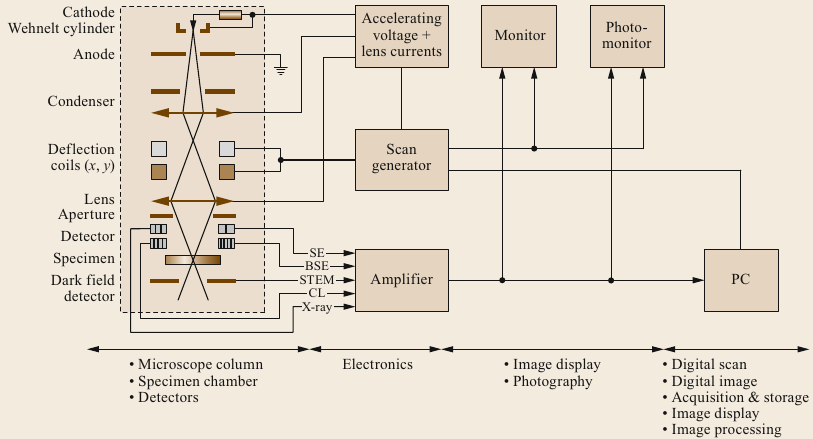
\includegraphics[width=0.65\textwidth]{img/sem_schematic}
    \caption{
    Schematische Darstellung eines konventionellen SEM.
    Die evakuierte Mikroskopsäule (im gestrichelten Rahmen) beinhaltet die Elektronenkanone, elektromagnetische Linsen, Blenden, Probenebene und Detektoren. \cite{springer-handbook}
    }
    \label{fig:sem_schematic}
\end{figure}

Im Folgenden soll der Fokus auf Sekundärelektronen und rückgestreute Elektronen gelegt werden.
Sekundärelektronen sind dadurch definiert, dass sie eine Energie von weniger als \SI{50}{eV} haben, während rückgestreute Elektronen darüber liegen.

Rückgestreute Elektronen werden zu einem kleinen Teil dadurch erklärt, dass ein kleiner Teil der Primärelektronen mit hohem Streuwinkel $\theta > \SI{90}{\degree}$ in Richtung Elektronenkanone zurückgestreut werden und dabei wenig bis keine Energie verlieren.
Da solche Streuprozesse jedoch relativ unwahrscheinlich sind, spielen im BSE-Signal Elektronen, die nach mehreren elastischen Streuprozessen die Probe verlassen die größere Rolle.
Je nach Probeneigenschaften und Primärenergie ergibt sich eine maximale Austrittstiefe, aus der Elektronen nachgewiesen werden können.
Üblicherweise befinden sich BSE-Detektoren auf einer Seite der Elektronenkanone, sodass Elektronen, die in diese Richtung austreten detektiert werden.
Da dies bei Oberflächen, die dem Detektor zugewandt sind, wahrscheinlicher ist, ergibt sich ein oberflächenorientierungsabhängiges Signal, das mit einem Schattenwurf in Lichtbildaufnahmen vergleichbar ist.
Außerdem nimmt die Wahrscheinlichkeit, dass Elektronen rückgestreut werden, mit der Ladungszahl zu, sodass BSE-Bilder chemischen Kontrast zeigen können (vgl. \cref{fig:bse-schatten}).

\begin{figure}[!ht]
    \centering
    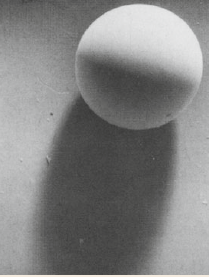
\includegraphics[width=0.65\textwidth]{img/bse-example}
    \caption{
     Backscattered electron micrograph of a 1-mm steel ball. \cite{springer-handbook}
    }
    \label{fig:bse-schatten}
\end{figure}

Sekundärelektronen entstehen durch inelastische Streuung von hochenergetischen Elektronen mit Probenatomen.
Hierbei wird Energie auf Elektronen in der Probe übertragen, welche aus ihrem Atompotenzial gelöst werden und danach die Energiedifferenz zwischen übertragener Energie und Ionisationsenergie als kinetische Energie besitzen.
Ist die kinetische Energie ausreichend groß und findet die Ionisation ausreichend nah an der Probenoberfläche statt, kann das Elektron die Probe verlassen und nachgewiesen werden. %2nm
Flächen, die nicht senkrecht zum Primärstrahl stehen begünstigen die Austrittswahrscheinlichkeit, wodurch SE-Bilder Informationen über die Topographie der Probe beinhalten.

Der Detektor kann sowohl das Objektivlinsensystem des Primärstrahls nutzen (through-the-lens detection) und somit parallel zum Primärstrahl messen oder seitlich montiert sein.
In beidem Fällen wird ein Spannungsgradient verwendet, um möglichst viele Elektronen \enquote{einzusammeln}.

\subsection{Probenpräparation für SEM}
%sample preperation requirements: vakuum, conductive for sem, thin for tem etc.
%Leitfähigkeit

\subsection{TEM}

Transmissionselektronenmikroskopie (TEM) erlaubt aufgrund der geringen Wellenlänge hochenergetischer Elektronen, Auflösungen zu erreichen, die mit Lichtmikroskopie aufgrund des Abbe-Limits unmöglich sind.
So kann mittels STEM (scanning transmission electron microscopy) in kristallinen Proben subatomare Auflösung, also die Visualisierung einzelner Orbitale, erreicht werden. %TODO kp, ob hier der Ausflug zu STEM Sinn ergibt.
Auch in biologischen Proben können Strukturen beobachtet werden, die im Lichtmikroskop nicht zugänglich sind. %TODO biologisch/organisch/?
Als Bild ergibt sich so auf dem Leuchtschirm ein Abbildung der Probe, in der für Elektronen schlecht durchlässige Bereiche dunkler als durchlässigere Bereiche erscheinen.
Im Allgemeinen sind Elemente höherer Ordnungszahl schlechter durchlässig.
%TODO Wenn der Typ STEM, Dunkelfeld gemacht hat oder sonst irgendwas spezielles, sollte ich das erwähnen, aber iirc hat er nicht.

\subsection{Probenpräparation für TEM}
%sample preperation requirements: vakuum, conductive for sem, thin for tem etc.

TEM erfordert im Gegensatz zu SEM extrem dünn geschnittene Proben (TODO), damit ausreichend viele Elektronen die Probe durchqueren, um ein Signal zu messen. %TODO welche Dicke etwa?
% Aufbringen auf Tem-Netze


\subsection{Astigmatismus} %TODO schauen, ob das Strukturell woanders besser passt und ob es ne eigene Überschrift braucht.

Astigmatismus tritt sowohl im TEM als auch im SEM auf, wenn Elektronen in unterschiedlichen Bildrichtungen eine unterschiedliche Fokusebene haben.
Astigmatismus entsteht durch Herrstellungsfehler in den Polstücken der Linsen.
Ein hoher Astigmatismus sorgt für eine Verzerrung oder Unschärfe des Bildes in einer Bildrichtung. \cite{MyScope}
Korrigieren lässt sich Astigmatismus durch Stigmatoren (Oktupole) in Kondensator- und Objektivlinsen, mithilfe deren man ein Feld aufbaut, das diese Herrstellungsfehler ausgleicht.

\section{Durchführung}

%actual sample preperation


%TEM:
%schwarze Punkte: schwere Elemente (OsO4 die ja vorher für Kontrast da reingepackt wurden).
	%sO4 gibt Kontraste für Lipide.
	%r mehr Kontraste: Urandingens, etc. => differential staining, differential contrast
